\def\duedate{10/14/22}
\def\HWnum{6}
% Document setup
\documentclass[12pt]{article}
\usepackage[margin=1in]{geometry}
\usepackage{fancyhdr}
\usepackage{lastpage}

\pagestyle{fancy}
\lhead{Richard Whitehill}
\chead{MATH 757 -- HW \HWnum}
\rhead{\duedate}
\cfoot{\thepage \hspace{1pt} of \pageref{LastPage}}

% Encoding
\usepackage[utf8]{inputenc}
\usepackage[T1]{fontenc}

% Math/Physics Packages
\usepackage{amsmath}
\usepackage{amssymb}
\usepackage{mathtools}
\usepackage[arrowdel]{physics}
\usepackage{siunitx}

\AtBeginDocument{\RenewCommandCopy\qty\SI}

% Reference Style
\usepackage{hyperref}
\hypersetup{
    colorlinks=true,
    linkcolor=blue,
    filecolor=magenta,
    urlcolor=cyan,
    citecolor=green
}

\newcommand{\eref}[1]{Eq.~(\ref{eq:#1})}
\newcommand{\erefs}[2]{Eqs.~(\ref{eq:#1})--(\ref{eq:#2})}

\newcommand{\fref}[1]{Fig.~\ref{fig:#1}}
\newcommand{\frefs}[2]{Figs.~\ref{fig:#1}--\ref{fig:#2}}

\newcommand{\tref}[1]{Table~\ref{tab:#1}}
\newcommand{\trefs}[2]{Tables~\ref{tab:#1}-\ref{tab:#2}}

% Figures and Tables 
\usepackage{graphicx}
\usepackage{float}

\newcommand{\bef}{\begin{figure}[h!]\begin{center}}
\newcommand{\eef}{\end{center}\end{figure}}

\newcommand{\bet}{\begin{table}[h!]\begin{center}}
\newcommand{\eet}{\end{center}\end{table}}

% tikz
\usepackage{tikz}
\usetikzlibrary{calc}
\usetikzlibrary{decorations.pathmorphing}
\usetikzlibrary{decorations.markings}
\usetikzlibrary{arrows.meta}
\usetikzlibrary{positioning}

% tcolorbox
\usepackage[most]{tcolorbox}
\usepackage{xcolor}
\usepackage{xifthen}
\usepackage{parskip}

\newcommand*{\eqbox}{\tcboxmath[
    enhanced,
    colback=black!10!white,
    colframe=black,
    sharp corners,
    size=fbox,
    boxsep=8pt,
    boxrule=1pt
]}

% Miscellaneous Definitions/Settings
\newcommand{\prob}[2]{\textbf{#1)} #2}
\newcommand{\reals}{\mathbb{R}}
\newcommand{\integers}{\mathbb{Z}}
\newcommand{\naturals}{\mathbb{N}}
\newcommand{\rationals}{\mathbb{Q}}
\newcommand{\complexs}{\mathbb{C}}

\setlength{\parskip}{\baselineskip}
\setlength{\parindent}{0pt}
\setlength{\headheight}{14.49998pt}
\addtolength{\topmargin}{-2.49998pt}







\begin{document}
    
\prob{1}{
Which operators are linear?
}

a) $\displaystyle Au = -\partial^2u$, $\mathcal{D} = \{ u \in C^2[0,\pi] ~\big|~ u(0) = 0 ~{\rm and}~ u'(\pi)=0 \}$

This is a linear operator on the vector space $\mathcal{D}$ since
\begin{eqnarray}
    \label{eq:lin-op-a}
    A(\alpha u + \beta v) = -\partial^2 (\alpha u + \beta v) = \alpha(-\partial^2 u) + \beta (-\partial^2 v) = \alpha Au + \beta Av
.\end{eqnarray}

b) $\displaystyle Au = -\partial^2u$, $\mathcal{D} = \{ u \in C^2[0,\pi] ~\big|~ u(0) = 0 ~{\rm and}~ u'(\pi)=\pi \}$

The space $\mathcal{D}$ is not a proper vector space since if $u,v \in \mathcal{D}$, then $u + v \not\in \mathcal{D}$ since $u'(\pi) + v'(\pi) = 2\pi$.
Hence, $A$ is not a linear operator on the space $\mathcal{D}$ since $Au$ must be in the vector space $\mathcal{D}$ for all $u \in \mathcal{D}$.

c) $\displaystyle Au = u_{xx} + x^2u$, $\mathcal{D} = C^2(\reals)$ 

This is clearly a linear operator since
\begin{eqnarray}
    \label{eq:lin-op-c}
    A(\alpha u + \beta v) = \partial_{x}^2(\alpha u + \beta v) + x^2(\alpha u + \beta v) = \alpha[u_{xx} + x^2u] + \beta[v_{xx} + x^2v] = \alpha Au + \beta Av
.\end{eqnarray}

d) $Au = u_{xx} + u^2$, $\mathcal{D} = C^2(\reals)$ 

This is not a linear operator:
\begin{eqnarray}
    \label{eq:lin-op-d}
    A(\alpha u) = \alpha u_{xx} + \alpha^2 u^2 \ne \alpha Au
.\end{eqnarray}


\prob{2}{
Solve $u_{t} = 3u_{x} + 5u$, $u(x,0) = f(x)$.
}

We wish to solve the equation $u_{t} = Au$, where $A = 3\partial_{x} + 5$ and $u(x,0) = f(x)$, which has solution 
\begin{eqnarray}
    \label{eq:solve-t-eq}
    \eqbox{
    u = e^{tA} f(x) = e^{3t\partial_{x}}e^{5t} f(x) = e^{5t}f(x+3t)
}
.\end{eqnarray}


\prob{3}{
    Solve $u_{tt} - u_{xx} = 0$, $x \in \reals$, $t > 0$ for $u(x,0) = 3\sin{5x} - \cos{3x}$, $u_{t}(x,0) = 2x + 3x^2$. Find only $u(0,t)$.
}

The general solution to the wave equation $u_{tt} - c^2u_{xx} = 0$ with initial conditions $u(x,0) = \phi(x)$, $u_{t}(x,0) = \psi(x)$ is
\begin{eqnarray}
    \label{eq:gen-sol-wave}
    u(x,t) = \frac{1}{2}\big[ \phi(x + ct) + \phi(x - ct) \big] + \frac{1}{2c} \int_{x-ct}^{x+ct} \psi(s) \dd{s}
.\end{eqnarray}
Hence, at $x = 0$, we have
\begin{align}
    \label{eq:x=0}
    u(0,t) &= \frac{1}{2} \big[ 3\sin{(5t)} - \cos{(3t)} - 3\sin{(-5t)} + \cos{(-3t)}] + \frac{1}{2}\int_{-t}^{t} (2s + 3s^2) \dd{s} \notag \\
           &= 3 \sin{(5t)} + \int_{0}^{t} 3s^2 \dd{s} \notag \\
           &= \eqbox{3\sin{(5t)} + t^3}
.\end{align}


\prob{4}{
Find $u(x,t)$ for the equation $u_{t} - ku_{xx} = 0$, $x \in \reals$, $t > 0$ subject to $u(x,0) = e^{-(x+1)^2}$.
}

We can find $u(x,t)$ subject to the initial condition as follows:
\begin{align}
    \label{eq:solve-u-diff}
    u(x,t) &= \frac{1}{\sqrt{4 \pi k t}} \int_{-\infty}^{\infty} e^{-(x-y)^2/4kt}e^{-(y+1)^2} \dd{y} \notag \\
           &= \frac{1}{\sqrt{4 \pi k t}} e^{-x^2/4kt - 1} \int_{-\infty}^{\infty} e^{-y^2/4kt - y^2 - 2y + xy/2kt} \dd{y} \notag \\
           &= \frac{1}{\sqrt{4 \pi k t}} e^{-x^2/4kt - 1} \int_{-\infty}^{\infty} e^{-(1 + 1/4kt)y^2 + 2(x/4kt - 1)y} \dd{y}
.\end{align}
Denote $a = 1 + 1/4kt$ and $b = x/4kt - 1$, then
\begin{align}
    \label{eq:u-diff-simplify}
    \int_{-\infty}^{\infty} e^{-(1 + 1/4kt)y^2 + 2(x/4kt - 1)y} \dd{y} &= \int_{-\infty}^{\infty} e^{-a(y^2 + 2by/a)} \dd{y} \notag \\
                                                                       &= e^{b^2/a} \int_{-\infty}^{\infty} e^{-a(y + b/a)^2} \dd{y} \notag \\
                                                                       &= e^{4kt(x/4kt - 1)^2/(1 + 4kt)} \sqrt{\frac{4 \pi k t}{1 + 4kt}}
.\end{align}
Finally, we have our solution:
\begin{eqnarray}
    \label{eq:solution-5}
    \eqbox{
    u(x,t) = \frac{1}{\sqrt{1 + 4kt}} e^{-(x+1)^2/(1 + 4kt)}
}
.\end{eqnarray}




\prob{5}{
    Find the Fourier transform $\displaystyle \widehat{f}(\omega) = \int_{-\infty}^{\infty} f(x)e^{-i\omega x} \dd{\omega}$ for $f(x) = xe^{-x^2}$.
}

The fourier transform of $f$ is given as
\begin{eqnarray}
    \label{eq:fourier-trans-f}
    \widehat{f}(\omega) = \int_{-\infty}^{\infty} xe^{-i\omega x} e^{-x^2} \dd{x} = \frac{i}{\omega} \dv{\omega} \int_{-\infty}^{\infty} e^{-i\omega x} e^{-x^2} \dd{\omega} = \frac{i}{\omega}\dv{\mathcal{F}\{\exp(-x^2)\}}{k}
.\end{eqnarray}
The fourier transform of this ``gaussian'' is as follows
\begin{align}
    \label{eq:fourier-trans-gauss}
    \mathcal{F}\{ e^{-x^2} \} &= \int_{-\infty}^{\infty} e^{-i\omega x} e^{-x^2} \dd{x} = \int_{-\infty}^{\infty} e^{-(x^2 + i\omega)} \dd{x} \notag \\
                              &= e^{-\omega^2/4} \int_{-\infty}^{\infty} e^{-(x + i\omega/2)^2} \dd{x} = \sqrt{\pi} e^{-\omega^2/4}
.\end{align}
Thus,
\begin{eqnarray}
    \label{eq:fourier-deriv}
\widehat{f}(\omega) = \frac{i\sqrt{\pi}}{\omega} \Big( -\frac{\omega}{2} e^{-\omega^2/4} \Big) = \eqbox{ -\frac{i\sqrt{\pi}}{2} e^{-\omega^2/4} }
.\end{eqnarray}


\prob{6*}{
    Find the Fourier transform for $f(x) = -H(x+1) + 2H(x) - H(x-1)$, where \\ $\displaystyle H(x) = \begin{cases} 1, & x \geq 0 \\ 0, & x < 0\end{cases}$.
}

Our function
\begin{eqnarray}
    \label{eq:f-piecewise}
    f(x) = 
    \begin{cases}
        -1 & -1 < x < 0 \\
        \phantom{-}1 &  \phantom{-}0 < x < 1 \\
        \phantom{-}0 &  \phantom{-}\mbox{otherwise}
    \end{cases}
.\end{eqnarray}
Therefore,
\begin{align}
    \label{eq:fourier-f}
    \widehat{f}(k) &= \int_{-\infty}^{\infty} e^{-ikx} f(x) \dd{x} = -\int_{-1}^{0} e^{-ikx} \dd{x} + \int_{0}^{1} e^{-ikx} \dd{x} \notag \\
                   &= \frac{1 - e^{ik}}{ik} - \frac{1 - e^{-ik}}{ik} = \frac{e^{-ik} - e^{ik}}{ik} = \eqbox{-\frac{2\sin{k}}{k}}
.\end{align}

\begin{figure}[H]
\begin{center}
    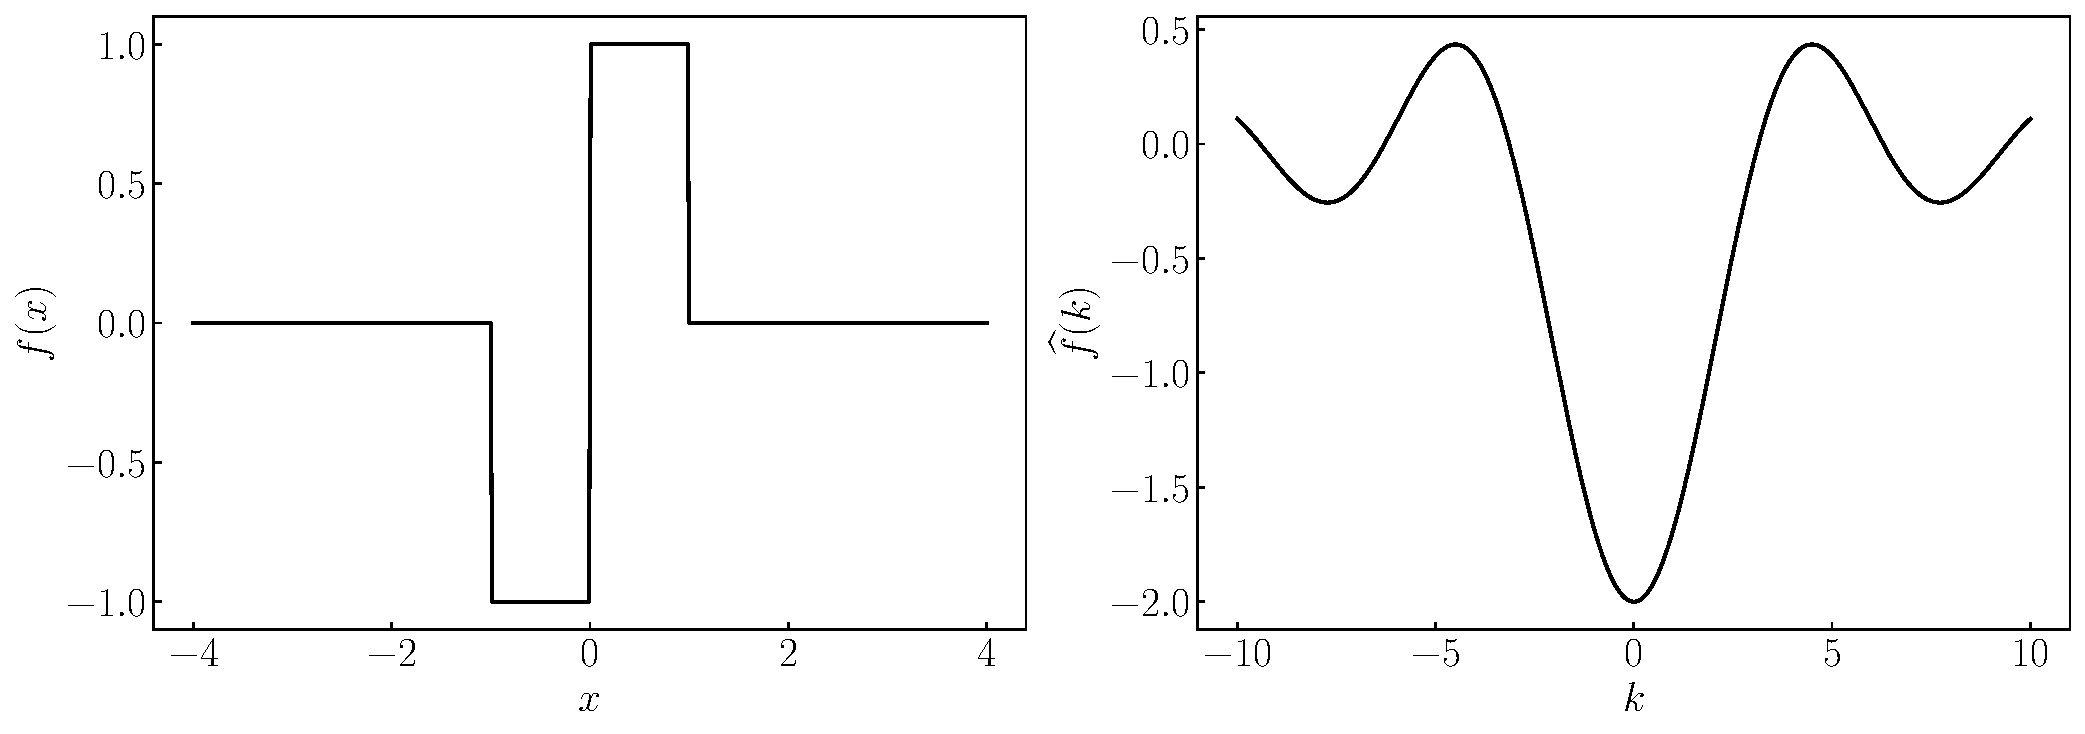
\includegraphics[width=\textwidth]{prob6.pdf} 
\end{center} 
\caption{
    Plot of $f(x)$ and the fourier transform $\widehat{f}(k)$.
}
\end{figure}


\prob{7*}{
Solve $u_{t} = 5u_{x} - 3xu + u$, $x \in \reals$, $t > 0$ with $u(x,0) = f(x)$.
}

We perform the change of variables $u = e^{\lambda x^2} v$, where $\lambda$ is a variable to be determined such that the equation becomes one that we know how to solve easily.
Then, the time and spatial derivatives are
\begin{align}
    \label{eq:change-vars}
    u_{t} &= e^{\lambda x^2} v_{t} \\
    u_{x} &= e^{\lambda x^2}( v_{x} + 2 \lambda x v)
.\end{align}
Our equation then becomes
\begin{eqnarray}
    \label{eq:change-vars-eq}
    \big[ v_{t} - 5v_{x} - 10 \lambda x v + 3xv - v \big] e^{\lambda x^2} = 0
.\end{eqnarray}
To simplify our calculation, we pick $\lambda = 3/10$, which gives $u = e^{3x^2/10}v$ and
\begin{eqnarray}
    \label{eq:change-vars-eq-2}
    v_{t} - 5v_{x} - v = v_{t} - Av = 0
,\end{eqnarray}
where $A = 5\partial_{x} + 1$.
This equation has solution
\begin{eqnarray}
    \label{eq:v-sol}
    v = e^{t(5 \partial_{x} + 1)}e^{-3x^2/10}f(x) = e^{t} e^{5t\partial_{x}}e^{-3x^2/10}f(x) = e^{t}e^{-3(x+5t)^2/10}f(x+5t)
,\end{eqnarray}
meaning
\begin{eqnarray}
    \label{eq:u-sol}
    \eqbox{
    u = e^{3x^2/10}e^{t}e^{-3(x+5t)^2/10}f(x+5t) = e^{-t(6x+15t-2)/2}f(x+5t)
}
.\end{eqnarray}







\end{document}
